\section{SYSTEM MODELS}
In order to determine the energy-efficient power budget of a multi-core dark silicon system, we present static power modeling and thermal modeling techniques in this section, which are important basic knowledges for our new work.

\subsection{Power modeling}

It is widely acknowledged that the total power of a chip is composed of dynamic and static power. The dynamic power is dependent on the activities of the chip, most of which is the capacitive switching power consumed during circuit charging and discharging. $p_{d}$ can be expressed in terms of the operating voltage $V_{dd}$, the clock frequency $f$, and the switching capacity $c$ as:
\begin{equation}\label{eq:dyn_power}
p_{d} = c \cdot V_{dd}^{2} \cdot f.
\end{equation}

It is assumed the clock frequency $f$ changes with $V_{dd}$ to the lowest allowable point:
\begin{equation}\label{eq:f_v}
f -f_{th}= (V_{dd}-V_{th}) \cdot (\frac{f_{max}-f_{th}}{V_{max}-V_{th}}).
\end{equation}

Yet the static power $p_{s}$ of the chip is caused by leakage current $I_{leak}$ as:
\begin{equation}\label{eq:sta_power}
p_{s} = V_{dd} \cdot I_{leak}.
\end{equation}
Due to the non-linear relationship between $I_{leak}$ and temperature, static power is also sensitive to temperature, which makes it hard to obtain. 

$I_{leak}$ is composed of many components, including subthreshold current, gate current, reverse-biased junction leakage current, et cetera. Among which, subthreshold current and gate current are the main parts of leakage current, therefore $I_{leak}$ can be approximated as:
\begin{equation}\label{eq:leakage}
I_{leak}=I_{sub}+I_{gate}.
\end{equation}

Noted that $I_{gate}$ is cause by tunneling between the gate terminal and the other three terminals, does not depend on temperature and can be considered as a technology-dependent constant. Yet $I_{sub}$ is considered to be highly related to temperature, and can be modeled in the commonly accepeted MOSFET transitor model BSIM 4 as:
\begin{equation}\label{eq:sub_current}\
I_{sub}=K {v_T}^2e^{\frac{V_{GS}-V_{th}}{\eta v_T}}
  (1-e^{\frac{-V_{DS}}{v_T}}) \approx K {v_T}^2e^{\frac{V_{GS}-V_{th}}{\eta v_T}},
\end{equation}

In xx, a local linearization of subthreshold current is implemented to eliminate the non-linear dependency of subthreshold current on temperature. The scalar result is
\begin{equation}\label{eq:lin_leakage}
p_{s} = V_{dd} \times (p_{0}+a_{s} \cdot T).
\end{equation}
$p_{0}$ is a constant terms that are not associated with $T$, $a_{s}$ is the coefficient associated with $T$. $P_{0}$ and $A_{s}$ are the constants corresponding for $p_{0}$ and $a_{s}$ in vector/matrix form.


%Apparently, the leakage current has a complex relationship with temperature. In this work, we use \eqref{eq:sta_power}, \eqref{eq:leakage}, and \eqref{eq:sub_current} to model the static power considering such relationship. The parameters of leakage current can be obtained by curve fitting using HSPICE simulation data. In order to see the accuracy of the model used, Fig.~\ref{fig:leakage} shows an HSPICE simulation result of leakage using TSMC \SI{65}{nm} process model and its curve fitting result using approximate leakage model. From the figure, we can see that the static power model has high accuracy for all common temperatures of IC chips.
% \begin{figure}%curve fitting
%   \centering
%   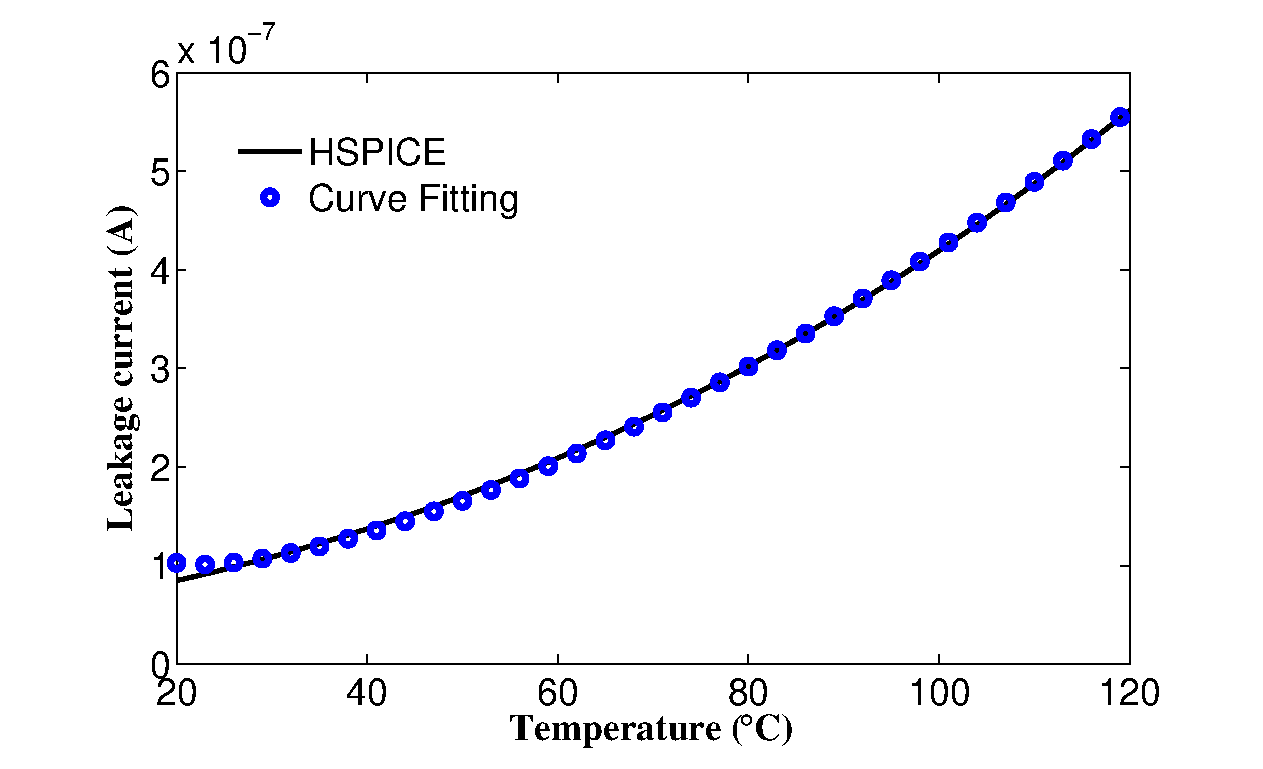
\includegraphics[width=1\columnwidth]{fig/leakage.eps}
%   \caption{Comparison of leakage of a TSMC \SI{65}{nm} process MOSFET from HSPICE
%     simulation with its curve fitting result using \eqref{eq:sub_current}. An example of
%     temperature region division is also shown in the figure, which will be discussed later.}
%   \label{fig:leakage}
% \end{figure}


\subsection{Thermal modeling}
In this work, the multi-core dark silicon system is packaged in a common structure in Fig. x. 
Heat (power) generated from the chip is conducted through thermal interface material (TIM), heat spreader, heat sink, and finally dissipated to the air through convection. The secondary heat path is ignored hear, since much fewer heat is dissipated through that path.

To estimate the power consumption of a IC chip, we first divide the chip and its package into multiple blocks called thermal nodes, with partition granularity determined by the accuracy requirements. For the dark silicon multi-core system (a 16-core chip's floorplan example is shown in Fig. x), we treat each core as a thermal node with a current source, because each core has very small area and highly correlated internal power distribution. The other thermal nodes from the package are divided according to the chip thermal nodes. Then, the thermal resistance and capacitance among these thermal nodes are determinded, which model the thermal transport and power response behaviors. Please note that multi-core system floorplan different from the one shown in Fig. x are fullly compatible with this work, and each core's internal structure can also be modeled if necessary. With above mentioned information, the thermal mdoel for a chip with $n$ total thermal nodes can be generated:
\begin{equation}\label{eq:gt}
\begin{split}
GT(t) + C\frac{dT(t)}{dt} &= BP(t)\\
T_{c}(t) &= B^{T}T(t)
\end{split}
\end{equation}
where $T(t) \in \mathbb{R}^m$ is the temperature rise vector , representing temperature rise (from the ambient temperature) at $m$ places of the chip and package; $G \in \mathbb{R}^{m\times m}$ and  $C \in \mathbb{R}^{m \times m}$ contain equivalent thermal resistance and capacitance information respectively; $B \in \mathbb{R}^{m \times n}$ stores the information of how powers are injected into the thermal nodes; $P(T, t) \in \mathbb{R}^{n}$ is the power vector, which contains power consumptions of $l$ components on chip, including both dynamic power vector $P_d$ and static power vector $P_s$, i.e., $P(T, t)=P_s(T, t)+P_d(t)$. $T_{c}(t) \in \mathbb{R}^n$ is the output temperature vector, containing only temperatures of cores only. For detailed structure of $G$, $C$, and $B$ matrices, please refer to the thermal modeling works such as xx.

With the model in \eqref{eq:gt}, the task of power budgeting is to determine the appropriate $P$, with a given temperature, to maximize the energy efficiency of the multi-core system, which is described next.